\documentclass[12pt]{article}
\usepackage{amssymb}
\usepackage{amsmath}
\usepackage{amsthm}
\usepackage{mathtools}
\usepackage{array}
\usepackage{multirow}
\usepackage{colortbl}
\usepackage[dvipsnames]{xcolor}
\usepackage{graphicx}
  \DeclareGraphicsRule{*}{mps}{*}{}
%\usepackage{bbm}
\usepackage{marvosym}
\usepackage{enumerate}
\usepackage{txfonts}
\usepackage{paralist}
\usepackage{pdfpages}
\usepackage{multicol}
\usepackage{tikz}
\usepackage{siunitx}
\usepackage[normalem]{ulem}
\everymath{\displaystyle}

\usepackage[margin=.7in]{geometry}
%\usepackage{fullpage}

\setdefaultleftmargin{0pt}{}{}{}{}{}

\newcommand{\mblank}{\rule[-1ex]{8ex}{0.4pt}}
\definecolor{lightgray}{gray}{0.7}

\newenvironment{solution}
{\color{BrickRed}\textbf{Solution.} 
}
{\ignorespacesafterend}

% Circles for Venn diagrams
\def\firstcircle{(90:1cm) circle (1.5cm)}
\def\secondcircle{(210:1cm) circle (1.5cm)}
\def\thirdcircle{(330:1cm) circle (1.5cm)}
% And here's the background rectangle
\def\universer{(-3, -2.5) rectangle (3, 2.75)}


\renewcommand{\thefootnote}{\fnsymbol{footnote}}

\hyphenpenalty=5000
\tolerance=1000
\setlength{\parindent}{0pt}

\begin{document}
\pagestyle{empty}


\section*{Reassessment Carnival Problems -- MATH 210 -- Spring 2019}

\begin{enumerate}

\item (\textbf{P1}) Here's a sketch of a proof of a theorem: if $n^2$ is a multiple of 5, then $n$ is a multiple of 5. The proof is by contrapositive: assume $n$ is not a multiple of 5. Then $n$ is of the form $5k + j$, where $k$ and $j$ are integers and $j = 1, 2, 3, 4$. Now we'd like to show $n^2$ is not a multiple of 5. $n^2 = (5k+j)^2 = 25k^2 + 10kj + j^2$. So then we can just look at what happens when we square $j$. The squares of 1, 2, 3, and 4 are all not multiples of 5 (we should check this). So you can't write $n^2$ as a multiple of 5 (we should check this too). Yay, we win.

Use the idea of this proof to show that if $n^2$ is divisible by 7, then $n$ is divisible by 7.


\item \textbf{(P2, L1)} Let $P(n)$ be the proposition ``$n$ is a prime number''. Consider the following statement: 
\[ \forall n \in \mathbb{N}, P(n) \to (\exists k\in \mathbb{N}, n = 2k+1). \]
This statement is false. Explain why, and give a counterexample.

\item \textbf{(P3)} Give a combinatorial proof of the fact that each row of Pascal's triangle adds up to a power of 2:
\[\binom{n}{0} + \binom{n}{1} + \ldots + \binom{n}{n} = 2^n. \]

\item \textbf{(P4)} The following is true for all integers $n \geq 1$. Prove it using mathematical induction.
\[\frac{1}{1 \cdot 2} + \frac{1}{2 \cdot 3} + ... + \frac{1}{n(n+1)}=\frac{n}{n+1}\]

\item \textbf{(P5)} Here is a true theorem: If $n^2$ is a multiple of 3, then $n$ is a multiple of 3. 

Here is an \textbf{incorrect} proof of this theorem:
\begin{quotation}
This proof is by contrapositive. Suppose that $n$ is not a multiple of 3. Then there is some integer $k$ such that $n = 3k + 1$. Therefore, $n^2 = (3k+1)^2 = 9k^2 + 6k + 1 = 3(3k^2 + 2k) + 1$. Let $\ell = 3k^2 + 2k$; then $\ell$ is also an integer. Thus $n^2 = 3\ell + 1$, and so $n^2$ is also not a multiple of 3. \qed
\end{quotation}
Explain why this proof is incorrect. For optional \textbf{P1} credit, fix this proof.


\item (\textbf{L1, L3}) Consider these two very similar-looking statements: 

$\exists x\in \mathbb{Z}\ \forall y \in \mathbb{Z}, x + y = 0$

$\forall y \in \mathbb{Z}\ \exists x\in \mathbb{Z}, x + y = 0$

\begin{enumerate}
    \item Translate both statements into words.
    \item Write in symbols the formal negation of both statements.
    \item Precisely one of these two statements is true. Which is it, and why?\\ (Moral: the order of quantifiers is super important.)
\end{enumerate}

\item (\textbf{L2}) We have a number of logical connectives but we really could have gotten away with fewer. For example, any time we wanted to say $P \iff Q$ we could have just said it with \textbf{AND}, \textbf{OR}, and \textbf{NOT} with $(P \land Q) \lor ( \lnot P \land \lnot Q)$. Write a truth table to show that these two statements are logically equivalent.


\item
\textbf{(L3, S4)} Consider the following statement about a relationship R on some set A:
        \[\exists x \in A \ \exists y \in A,\ xRy \land \lnot (yRx) \]
\begin{enumerate}
    \item 
    Write the formal simplified negation of this statement.
    \item
    Explain the meaning of the original statement and the meaning of its negation using familiar properties of relations.
\end{enumerate}

\item \textbf{(S1, S2)} Consider the sets $A = \{a\in\mathbb{N}: \exists k\in\mathbb{N}, a = 5k\}$ and $B = \{b\in\mathbb{N}: \exists j\in\mathbb{N}, b = 6j+1\}$.
\begin{enumerate}
    \item Give an example of some number in $A\cap B$. Explain why you're right.
    \item Give an example of some number in $A\cap\overline{B}$. Explain why you're right.
\end{enumerate}

\item \textbf{(S3)} Another way functions (and more general relations) are sometimes represented is as a set of ordered pairs. For instance, if $f:\{1,2,3,4\}\to\mathbb{N}$ was given by $f(x) = x^2$, then we could write $f$ as the set $\{(1,1), (2,4), (3,9), (4, 16)\}$.

\begin{enumerate}
\item Let $g:\{a,b,c,d\}\to\{v,w,x,y,z\}$  be given by the set of ordered pairs \[\{(d,v), (a,x), (c,y), (b,w), (a,x), (c,z), (d,v)\}.\] Is $g$ a function? Why or why not?
\item Let $h:\{a,b,c,d\}\to\{v,w,x,y,z\}$ be given by the set of ordered pairs \[\{(c,x),(d,y),(a,y),(c,x),(b,z)\}.\]
I'll tell you for free that $h$ is a function. Is it injective? Is it surjective? Explain why or why not.
\end{enumerate}

\item \textbf{(S4, S5)}  Recall that the power set of $A$, written $\mathcal{P}(A)$, is the set of all subsets of $A$.

\begin{enumerate}
    \item Write all of the elements of $\mathcal{P}(\{1,2,3\})$.
    \item We define a relation on $\mathcal{P}(\{1,2,3\})$ as follows: For all sets $X$ and $Y$ in the power set, $X$ is related to $Y$ if and only if $X$ and $Y$ have the same cardinality. Explain why this relation is reflexive, symmetric, and transitive (thus, is an equivalence relation).
    \item Write the equivalence classes for this relation.
    
\end{enumerate}

\item \textbf{(C1, C3)} Suppose you have a huge box of animal crackers containing plenty of each of 10 different animals. Write a counting problem about giving animal crackers to people whose answer is $\textstyle\binom{10}{6}$, and carefully explain why the answer to your problem is $\textstyle\binom{10}{6}$.

\item \textbf{(C2)} Consider five-digit numbers $a = a_1 a_2 a_3 a_4 a_5$, where each digit $a_i$ comes from the set $\{1,2,3,4\}$. How many such numbers contain more even digits than odd digits? Carefully explain your answer.

\item (\textbf{Q1}) Find $3 + 7 + 11 + 15 + \cdots + 427$. Show all your work.

\item \textbf{(Q1, Q2)} Recall that $K_{n}$ is the complete graph on $k$ vertices. Consider the sequence defined below on all natural numbers $n \geq 1$:
\begin{center}
$s_{n}$ is the number of edges in $K_{n}$
\end{center}

\begin{enumerate}
    \item Find $s_{1}$, $s_{2}$, $s_{3}$, $s_{4}$, and $s_{5}$.
    \item Find a recurrence relation for $s_{n}$.
    \item Find a closed formula for $s_{n}$.
\end{enumerate}

\item \textbf{(G1, G3)} The city of Queenigsberg spans both sides of a river and includes three islands with bridges as shown below. (Picture from Epp 2011)

\begin{center}
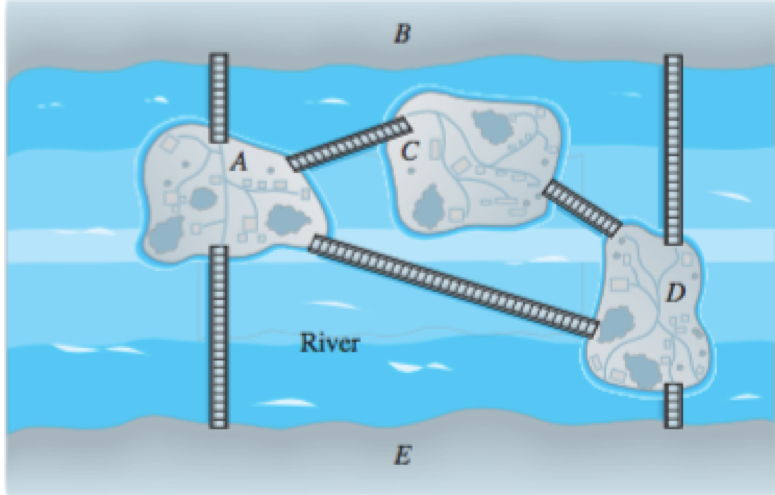
\includegraphics[width=0.5\textwidth]{bridge_picture.png}
\end{center}

\begin{enumerate}
    \item Draw a graph accurately representing the city and its bridges.
    \item Is it possible to take a walk around the city starting and ending at the same point and crossing each bridge exactly once? Explain.
\end{enumerate}

\item \textbf{(G2)} Draw two non-isomorphic graphs with 4 vertices. Carefully explain how you know they are not isomorphic.

\item \textbf{(G3)} Is it possible for a citizen of  K\"{o}nigsberg to go on a walking tour of the city crossing each bridge exactly twice? Explain.

\item \textbf{(G4)} Draw a graph with 7 vertices that has a chromatic number of 5.

%%%%%%%%%%%%%%%%%%%%%%%%%%%%%%%%%%%%%%%%%%%%%%%%%%%%%%%%%%%%%%%%%%%%%%%%%%%%%%%%%%%%%
\end{enumerate}
\end{document}